\documentclass[a4paper, 12pt]{article}

\usepackage{cmap}
\usepackage[T2A]{fontenc}
\usepackage[utf8]{inputenc}
\usepackage[english, russian]{babel}

%Графика
\usepackage{graphicx}
\usepackage{float}%"Плавающие" картинки
\usepackage{wrapfig}%Обтекание фигур (таблиц, картинок и прочего)
\graphicspath{{./images/}}

% Математика
\usepackage{amsmath,amsfonts,amssymb,amsthm,mathtools} 

%Title Page
\title{ЛАБОРАТОРНАЯ РАБОТА № 1 \\
МОДЕЛИРОВАНИЕ ЛИНЕЙНЫХ ДИНАМИЧЕСКИХ
СИСТЕМ
}
\author{Вариант 11 \\ Машуров Владимир БПМ-19-3}

\setcounter{page}{0}

\begin{document}
\maketitle
\thispagestyle{empty}
\newpage
\tableofcontents

\section{Исследование модели вход-выход}

Дано: $ n = 2 $, $ a_0 = 30 $, $  a_1 = 0.8 $, $  b_0 = 8 $, $  b_1 = 3 $ \\
Модель вход-выход имеет вид:
$$ \ddot{y} + 0,8\dot{y}+30y=3\dot{U} + 30U $$
Представим его в операторной форме приняв $s=\frac{d}{dt}$
$$ s^2y + 0,8sy + 30y = 3sU + 30U $$
$$ y = \frac{1}{s^2}(30U - 30y) + \frac{1}{s}(3U - 0,8y) $$
В полученной записи легко представить модель в виде схемы с помощью программы \textit{Scilab}, результат можно увидеть на картинке \ref{p:Схема1}.

\begin{figure}[h!]
	\centering
	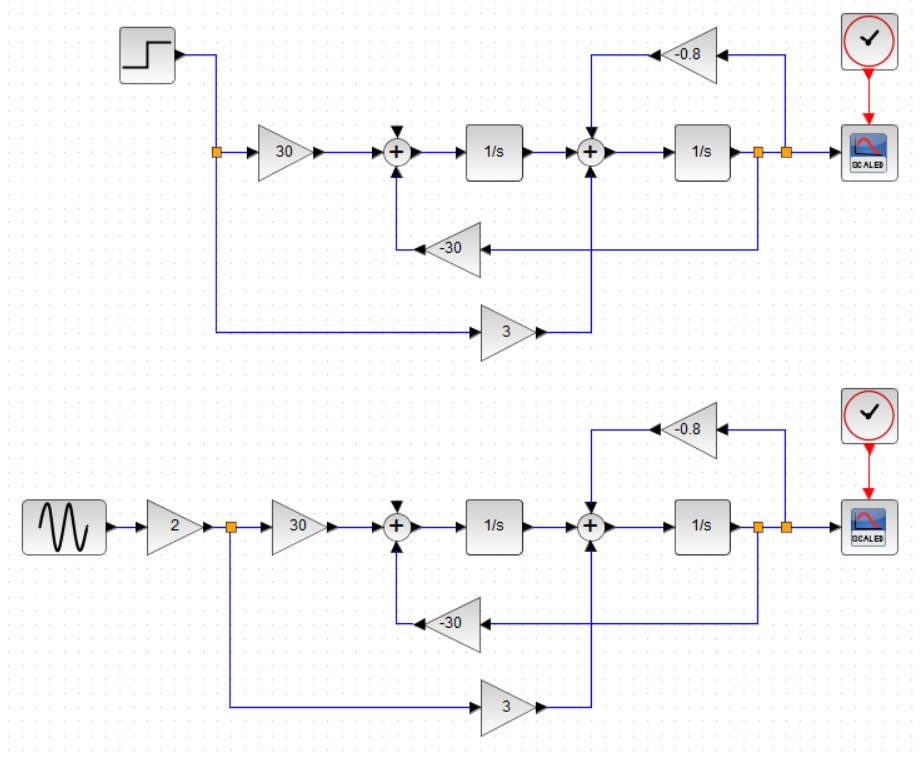
\includegraphics[scale=0.52]{scheme1}
	\caption{Схема математической модели в \textit{Scilab}}
	\label{p:Схема1}
\end{figure}   

На картинке \ref{p:Схема1} сверху и снизу представлена одна и та же модель, но с разными входными воздействиями. Вверху это $U = \begin{cases} 1, x \geq 1 \\ 0, x < 1 \end{cases}$, а внизу $U = 2\sin(t)$ 

На рисунках \ref{p:График1_1} и \ref{p:График1_2} можно увидеть графики модели при разных входных воздействиях, соответственно сверху - входное воздействие, снизу - реакция системы. Продолжительность интервала наблюдений по умолчанию.

\begin{figure}[h!]
	\centering
	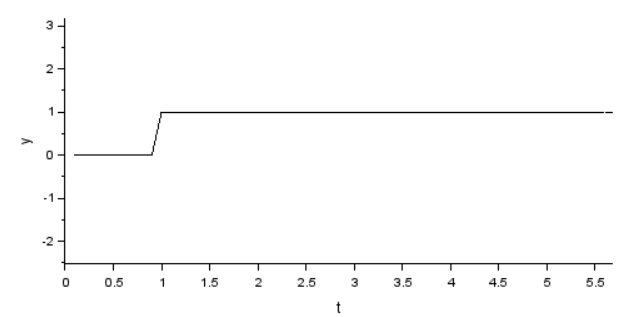
\includegraphics[scale=0.7]{plot1_3}
	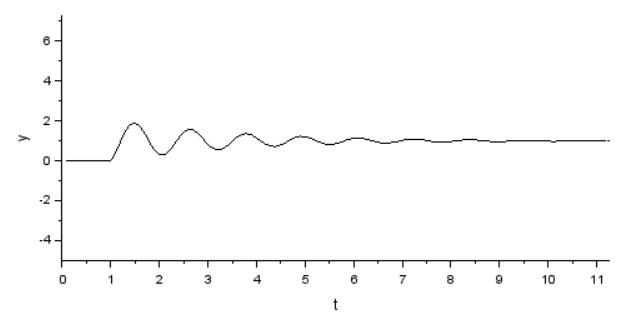
\includegraphics[scale=0.7]{plot1_1}
	\caption{График при нулевых начальных условиях  и входным воздействием $1(t)$ }
	\label{p:График1_1}
\end{figure}  

\begin{figure}[h!]
	\centering
	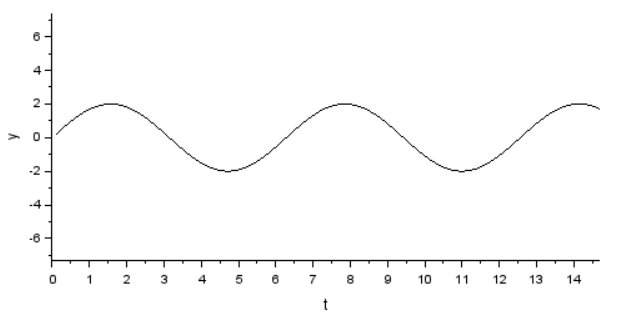
\includegraphics[scale=0.7]{plot1_4}
	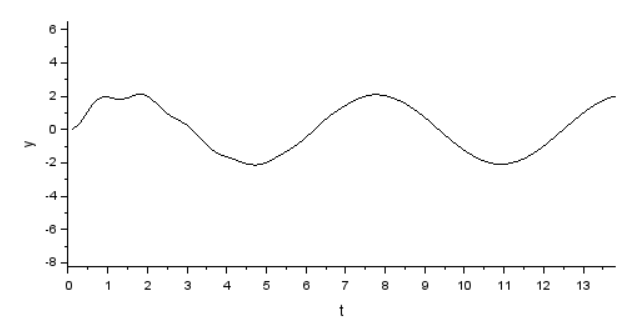
\includegraphics[scale=0.7]{plot1_2}
	\caption{График при нулевых начальных условиях и входным воздействием $2\sin(t)$ }
	\label{p:График1_2}
\end{figure}  

Даля моделирования свободного движения системы были даны начальные условия: $n=2$, $y(0)=1$, $\dot{y}(0)=0.5$ 

На рисунке \ref{p:Схема2} показана схема моделирования свободного движения. Там же можно увидеть $ z_1, \dot{z_1}, z_2, \dot{z_2} $ наглядно на схеме модели.

Проведём преобразования: 

$$ y = z_1 \Rightarrow \dot{y} = \dot{z} = z_2 +3U - 0.8y $$
Отсюда:
$$ \ddot{y} = \ddot{z_2} + 3\dot{U} -0,8\dot{y} = 30U - 30y - 0,8\dot{y}$$ 

Из полученных равенств получим значения для $z_1(0)$ и $z_2(0)$:

$$ y(0) = z_1(0) = 1 $$

$$ \dot{y}(0) = \dot{z_1}(0) = z_2(0) + 3U(0) - 0,8y(0) = 0,5 $$

Заметим, что $U(0)=0$

$$ z_2(0) + 3 \times 0 - 0,8 \times 1 = 0,5 \Rightarrow z_2(0) = 1,3 $$

\begin{figure}[h!]
	\centering
	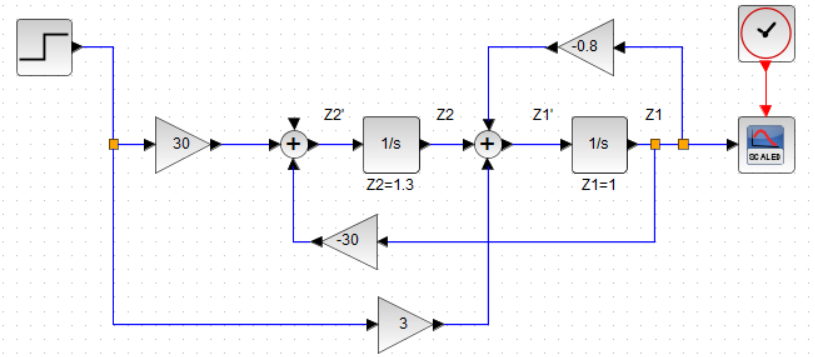
\includegraphics[scale=0.6]{scheme2}
	\caption{Схема моделирования свободного движения системы}
	\label{p:Схема2}
\end{figure}

На рисунке \ref{p:График2} показаны графики нулевого входного воздействия, снизу, и реакции системы, сверху.

\begin{figure}[h!]
	\centering
	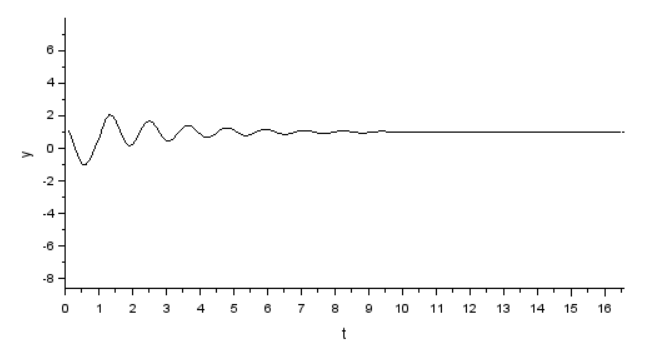
\includegraphics[scale=0.7]{plot2}
	\caption{График при моделировании свободного движения системы}
	\label{p:График2}
\end{figure}

\newpage
\section{Исследование модели вход-состояние-выход}

Дано: \\
\begin{center}
$ A = \begin{vmatrix}
0 & 1 & 1\\
-4 & -1 & 2\\
0 & 1 & -2
\end{vmatrix}  $
$ B = \begin{vmatrix}
0\\ 2\\ 1
\end{vmatrix}
$
$ C^T = \begin{vmatrix}
1\\ 0\\ 0.5
\end{vmatrix} $
\end{center}

Начальные условия системы: \\
$$ x_1(0)=0.5, \;  x_2(0)=-2, \; x_3(0)=0 $$

Из условий запишем систему:
$$ \begin{cases} \dot{x_1} = x_2 + x_3 \\ 
\dot{x_2} = -4x_1 - x_2 + 2x_3 + 2U \\
\dot{x_3} = x_2 - 2x_3 + U \\
y = x_1 + 0.5x_3 \end{cases} $$

Построим получившуюся систему в \textit{Scilab} (смотреть рисуноки \ref{p:ГрафикВСВ1} и \ref{p:ГрафикВСВ2}):

\begin{figure}[h!]
	\centering
	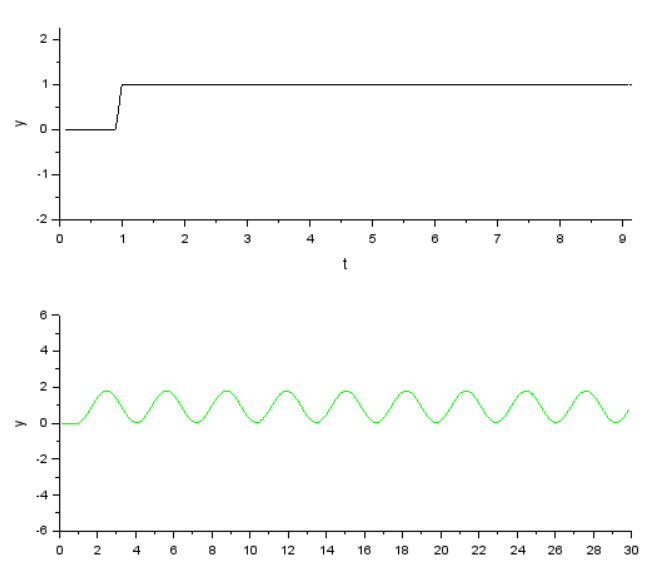
\includegraphics[scale=0.7]{plot2_1}
	\caption{График при моделировании системы вход-состояние-выход при нулевых начальных условиях и входным воздействием $1(t)$}
	\label{p:ГрафикВСВ1}
\end{figure}

\begin{figure}[h!]
	\centering
	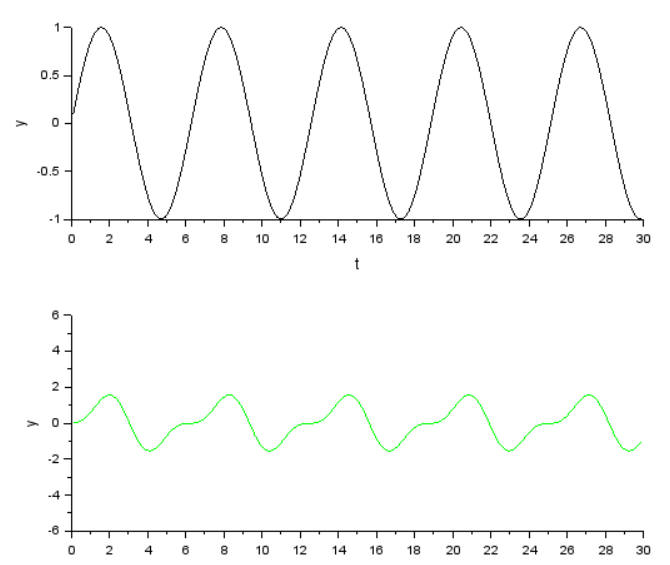
\includegraphics[scale=0.7]{plot2_2}
	\caption{График при моделировании системы вход-состояние-выход при нулевых начальных условиях и входным воздействием $2\sin{t}$}
	\label{p:ГрафикВСВ2}
\end{figure}

Произведём вычисления значений интеграторов для моделирования свободного движения системы:
$$ y(0) = x_1(0) + 0.5x_3(0) = 0.5 $$
$$ \dot{x_1}(0) = x_2(0) + x_3(0) = -2 + 0 = -2 $$
$$ \dot{x_3}(0) = x_2(0) - 2x_3(0) + U(0) = -2 - 2 \times 0 + 0 = -2 $$
$$ \dot{x_2}(0) = -4x_1(0) - x_2(0) + 2x_3(0) + 2U(0) = -4 \times 0.5 + 2 + 2 \times 0 + 2 \times 0 = -2 + 2 + 0 + 0 = 0 $$

График реакции системы $y$ можно увидеть на рисунке \ref{p:ГрафикВСВсвобода}.

\begin{figure}[h!]
	\centering
	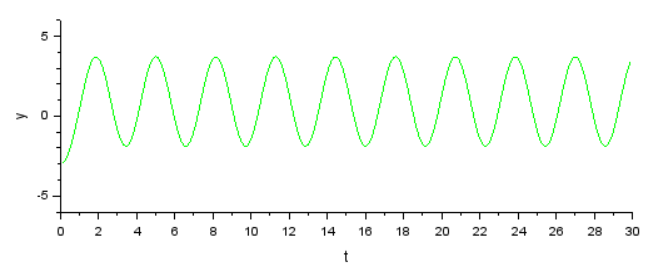
\includegraphics[scale=0.7]{plot2_3}
	\caption{График реакции системы при моделировании свободного движения системы вход-состояние-выход}
	\label{p:ГрафикВСВсвобода}
\end{figure}

Сама система выглядит следующим образом (смотреть рисунок \ref{p:Схема3}).

\begin{figure}[h!]
	\centering
	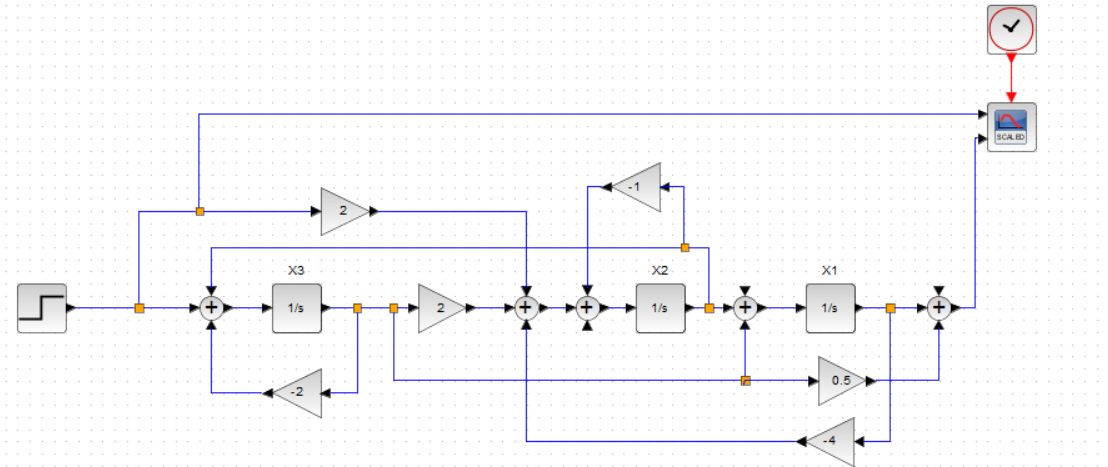
\includegraphics[scale=0.6]{scheme3}
	\caption{Схема моделирования системы}
	\label{p:Схема3}
\end{figure}

При моделировании системы с входным воздействием $2 \sin{t}$ - блок ступенчатого воздействия заменяется на последовательность блоков функции синуса и блока gain со значением 2.

\end{document}